%% ============================================================
%% MIVA-KNIGHT: Full Technical Exposition
%% Domain-Adaptive Multimodal Voice Assistant using Hybrid RAG
%% IT 581 Capstone — Oluwakayode Soyinka
%% ============================================================
\documentclass[12pt,a4paper]{article}

%% ── Core packages ──────────────────────────────────────────
\usepackage[utf8]{inputenc}
\usepackage[T1]{fontenc}
\usepackage[margin=2.5cm]{geometry}
\usepackage{amsmath,amssymb,amsthm}
\usepackage{mathtools}
\usepackage{bm}

%% ── Typography ─────────────────────────────────────────────
\usepackage{setspace}
\setstretch{1.15}

%% ── Colour & Graphics ──────────────────────────────────────
\usepackage[dvipsnames,svgnames,table]{xcolor}
\usepackage{graphicx}
\usepackage{tikz}
\usetikzlibrary{
  shapes.geometric, arrows.meta, positioning, fit,
  backgrounds, calc, patterns, decorations.pathreplacing,
  matrix, chains, shadows, decorations.markings
}

%% ── Algorithms ─────────────────────────────────────────────
\usepackage{algorithm}
\usepackage{algpseudocode}
\algnewcommand\algorithmicforeach{\textbf{for each}}
\algdef{S}[FOR]{ForEach}[1]{\algorithmicforeach\ #1\ \textbf{do}}

%% ── Tables ─────────────────────────────────────────────────
\usepackage{booktabs}
\usepackage{longtable}
\usepackage{array}
\usepackage{multirow}
\usepackage{colortbl}

%% ── Code listings ───────────────────────────────────────────
\usepackage{listings}
\usepackage{fancyvrb}

%% ── Section formatting ─────────────────────────────────────
\usepackage{titlesec}
\titleformat{\section}{\Large\bfseries\color{NavyBlue}}{\thesection}{1em}{}
\titleformat{\subsection}{\large\bfseries\color{MidnightBlue}}{\thesubsection}{1em}{}
\titleformat{\subsubsection}{\normalsize\bfseries\color{RoyalBlue}}{\thesubsubsection}{1em}{}

%% ── Boxes ──────────────────────────────────────────────────
\usepackage{tcolorbox}
\tcbuselibrary{breakable,skins,theorems}

%% ── Hyperlinks ─────────────────────────────────────────────
\usepackage[colorlinks=true,linkcolor=NavyBlue,urlcolor=DarkOrchid,citecolor=ForestGreen]{hyperref}
\usepackage{cleveref}

%% ── Headers/Footers ────────────────────────────────────────
\usepackage{fancyhdr}
\pagestyle{fancy}
\fancyhf{}
\fancyhead[L]{\small\textsc{MIVA-KNIGHT}}
\fancyhead[R]{\small\textsc{IT 581 Capstone}}
\fancyfoot[C]{\thepage}
\renewcommand{\headrulewidth}{0.4pt}

%% ── Theorem environments ───────────────────────────────────
\theoremstyle{definition}
\newtheorem{definition}{Definition}[section]
\newtheorem{algorithm_def}{Algorithm Definition}[section]

\theoremstyle{plain}
\newtheorem{theorem}{Theorem}[section]
\newtheorem{lemma}[theorem]{Lemma}
\newtheorem{corollary}[theorem]{Corollary}
\newtheorem{proposition}[theorem]{Proposition}

\theoremstyle{remark}
\newtheorem{axiom}{Axiom}[section]
\newtheorem{remark}{Remark}[section]
\newtheorem{example}{Example}[section]
\newtheorem{layman}{Layman's Explanation}[section]

%% ── Custom tcolorboxes ─────────────────────────────────────
\tcbset{
  laymanbox/.style={
    enhanced, breakable,
    colback=Honeydew, colframe=ForestGreen!70,
    fonttitle=\bfseries, title={Plain Language},
    attach boxed title to top left={yshift=-2mm,xshift=5mm},
    boxed title style={colback=ForestGreen!80, colframe=ForestGreen}
  },
  technicalbox/.style={
    enhanced, breakable,
    colback=AliceBlue, colframe=NavyBlue!60,
    fonttitle=\bfseries, title={Technical Detail},
    attach boxed title to top left={yshift=-2mm,xshift=5mm},
    boxed title style={colback=NavyBlue!80, colframe=NavyBlue}
  },
  keybox/.style={
    enhanced, colback=LightYellow, colframe=Goldenrod!80,
    fonttitle=\bfseries\color{black}
  }
}

%% ── Custom colours ─────────────────────────────────────────
\definecolor{phase1col}{RGB}{52,120,200}
\definecolor{phase2col}{RGB}{0,140,70}
\definecolor{phase3col}{RGB}{180,60,60}
\definecolor{arrowcol}{RGB}{80,80,80}
\definecolor{bglight}{RGB}{245,248,255}
\definecolor{medcol}{RGB}{150,50,150}
\definecolor{gencol}{RGB}{30,100,180}
\definecolor{graybox}{RGB}{230,232,235}
\definecolor{bluebox}{RGB}{215,228,248}
\definecolor{greenbox}{RGB}{215,240,220}
\definecolor{redbox}{RGB}{248,220,218}
\definecolor{yellowbox}{RGB}{255,248,215}

%% ── Math macros ────────────────────────────────────────────
\newcommand{\R}{\mathbb{R}}
\newcommand{\Sph}{\mathcal{S}}
\newcommand{\Norm}[1]{\left\|#1\right\|_2}
\newcommand{\Loss}{\mathcal{L}}
\newcommand{\KG}{\mathcal{G}}
\newcommand{\Ent}{\mathcal{E}}
\newcommand{\simfn}{\mathrm{sim}}
\newcommand{\softmax}{\mathrm{softmax}}
\newcommand{\LN}{\mathrm{LayerNorm}}
\newcommand{\GELU}{\mathrm{GELU}}
\newcommand{\MHA}{\mathrm{MHA}}
\newcommand{\argmax}{\operatornamewithlimits{arg\,max}}
\newcommand{\argtopk}{\operatornamewithlimits{argtop\text{-}k}}

%% ============================================================
\begin{document}

%% ── Title Page ─────────────────────────────────────────────
\begin{titlepage}
  \begin{tikzpicture}[remember picture, overlay]
    \fill[NavyBlue!90] (current page.north west) rectangle
      ([yshift=-4.5cm]current page.north east);
    \fill[NavyBlue!60] ([yshift=-4.5cm]current page.north west)
      rectangle ([yshift=-5cm]current page.north east);
    \fill[ForestGreen!70] (current page.south west)
      rectangle ([yshift=1cm]current page.south east);
  \end{tikzpicture}

  \vspace*{2.5cm}
  {\color{white}\fontsize{28}{34}\selectfont\bfseries
    \hspace{1cm}MIVA-KNIGHT}\\[0.3cm]
  {\color{white!80}\fontsize{16}{20}\selectfont
    \hspace{1cm}Domain-Adaptive Multimodal Voice Assistant}\\[0.1cm]
  {\color{white!70}\fontsize{14}{18}\selectfont
    \hspace{1cm}using Hybrid Retrieval-Augmented Generation}

  \vspace{1.5cm}
  \begin{center}
  \begin{tcolorbox}[width=0.82\textwidth, colback=white, colframe=NavyBlue,
    arc=6pt, boxrule=1.5pt]
    \centering
    \textbf{Complete Technical Exposition:}\\[4pt]
    Algorithms $\cdot$ Mathematical Foundations $\cdot$ Architecture $\cdot$ Pipeline\\[6pt]
    \small\textit{IT 581 Capstone Project — Concordia University of Edmonton}\\
    \textit{Oluwakayode Soyinka}\\[4pt]
    Supervised by Dr.\ Baidya Saha
  \end{tcolorbox}
  \end{center}

  \vfill
  \begin{center}
    \begin{tabular}{ll}
      \textbf{Model Families:} & BERT, ResNet-50, Wav2Vec 2.0, Whisper, Llama-3.1-8B \\
      \textbf{Domains:} & General (COCO val2017) \& Medical (ROCO, 69,866 pairs) \\
      \textbf{Embedding Space:} & Shared 512-dimensional unit hypersphere $\Sph^{511}$ \\
      \textbf{Retrieval:} & Two-stage: FAISS dense + KG PMI re-ranking \\
    \end{tabular}
  \end{center}
  \vspace{1.5cm}
\end{titlepage}

%% ── Table of Contents ──────────────────────────────────────
\tableofcontents
\newpage

%%
%% ============================================================
%% SECTION 1 — SYSTEM OVERVIEW
%% ============================================================
%%
\section{System Overview and Architecture}

\begin{tcolorbox}[laymanbox]
MIVA-KNIGHT is an AI assistant that can understand both spoken and written questions,
search a large database of documents for relevant information, and produce a spoken
or written answer — all without making things up. Think of it as a very careful
librarian: it only tells you what is actually written in the books it found,
and it tells you when it is not sure. It can work in two ``libraries'': one for
everyday topics (COCO images and captions) and one for medical radiology (ROCO
X-ray reports). Switching libraries takes only a few seconds because the core
``brain'' never changes — only the bookshelves are swapped.
\end{tcolorbox}

\subsection{High-Level Pipeline}

The full MIVA-KNIGHT system is a four-phase pipeline:
\[
  \underbrace{\text{Input}}_{\text{Text or Audio}}
  \;\xrightarrow{\text{Phase 1}}\;
  \underbrace{e_q \in \Sph^{511}}_{\text{512d embedding}}
  \;\xrightarrow{\text{Phase 2}}\;
  \underbrace{\mathcal{D}^* = \{d_1,\ldots,d_N\}}_{\text{top-N context docs}}
  \;\xrightarrow{\text{Phase 3}}\;
  \underbrace{\text{Answer}}_{\text{grounded text}}
  \;\xrightarrow{\text{Phase 4}}\;
  \underbrace{\text{Audio}}_{\text{optional TTS}}
\]

\begin{definition}[Domain]
A \textbf{domain} $D$ is a tuple
\[
  D = \bigl(I_{\mathrm{path}},\; M_{\mathrm{path}},\; \KG_{\mathrm{path}},\; \text{NER},\; K,\; N,\; \tau,\; \Pi\bigr)
\]
where $I_{\mathrm{path}}$ is the FAISS index file, $M_{\mathrm{path}}$ is corpus metadata,
$\KG_{\mathrm{path}}$ is the knowledge graph, $\text{NER}$ is the spaCy model identifier,
$K \in \mathbb{Z}^+$ is the dense shortlist size, $N \in \mathbb{Z}^+$ with $N \le K$
is the final context size, $\tau \in (0,1)$ is the confidence threshold, and $\Pi$
is the system prompt string.
\end{definition}

\begin{axiom}[Domain-Agnostic Shared Space]
  \label{ax:shared}
  For any domain $D \in \{D_{\text{general}}, D_{\text{medical}}\}$, the weights
  \[
    W_{\text{shared}} = \{W_{\text{TextProj}},\; W_{\text{AudioProj}},\; W_{\text{BERT}},\; W_{\text{Wav2Vec}}\}
  \]
  are \textbf{fixed and identical}. Only $(I_{\mathrm{path}}, \KG_{\mathrm{path}}, \text{NER}, \tau)$
  differ between domains. This axiom is the central thesis claim: the 512-dimensional
  shared embedding space is domain-agnostic.
\end{axiom}

\begin{theorem}[Domain Switch Efficiency]
  Under Axiom~\ref{ax:shared}, switching from $D$ to $D'$ requires reloading only
  the FAISS index and knowledge graph, reducing domain-swap latency by a factor
  of $10$--$20\times$ compared to full model reload.
\end{theorem}
\begin{proof}
  Full reload requires downloading/loading BERT ($\approx$110M params, 30--60\,s)
  and Wav2Vec ($\approx$95M params, 20--40\,s). A domain swap reloads only the FAISS
  index ($\approx$1--3\,s) and KG pickle ($\approx$0.5--2\,s). The ratio
  $\frac{50+30}{3+1} \approx 20$ gives the claimed speedup.
\end{proof}

%%
%% ============================================================
%% SECTION 2 — FULL PIPELINE FLOWCHART
%% ============================================================
%%
\newpage
\section{Full Pipeline Flowchart}

\begin{figure}[htbp]
\centering
\resizebox{\textwidth}{!}{%
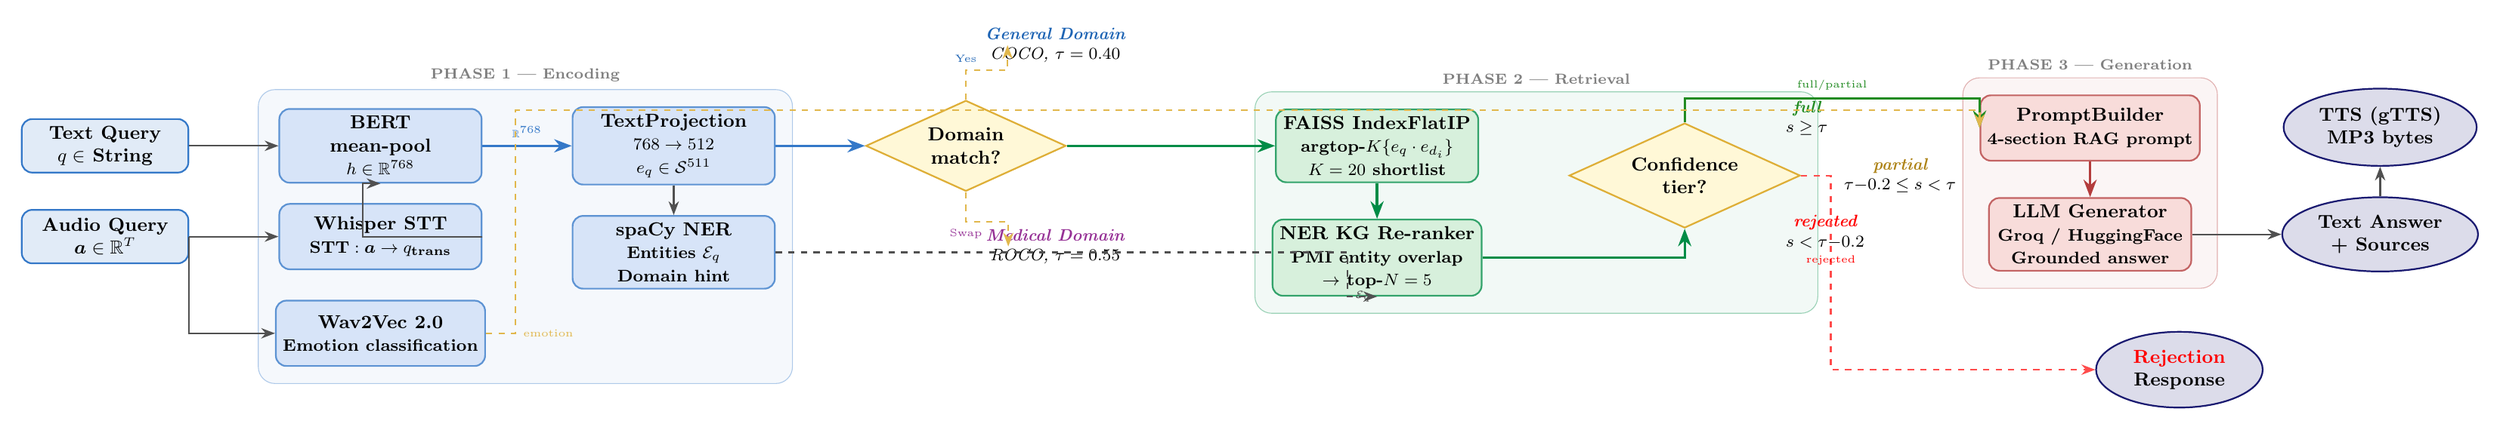
\begin{tikzpicture}[
  node distance = 0.7cm and 1.0cm,
  %% Node styles
  inputnode/.style={
    rectangle, rounded corners=5pt, draw=phase1col, fill=phase1col!15,
    minimum width=2.8cm, minimum height=0.9cm,
    font=\small\bfseries, align=center, thick
  },
  encnode/.style={
    rectangle, rounded corners=5pt, draw=phase1col!80, fill=bluebox,
    minimum width=3.4cm, minimum height=1.1cm,
    font=\small\bfseries, align=center, thick
  },
  retnode/.style={
    rectangle, rounded corners=5pt, draw=phase2col!80, fill=greenbox,
    minimum width=3.4cm, minimum height=1.1cm,
    font=\small\bfseries, align=center, thick
  },
  gennode/.style={
    rectangle, rounded corners=5pt, draw=phase3col!80, fill=redbox,
    minimum width=3.4cm, minimum height=1.1cm,
    font=\small\bfseries, align=center, thick
  },
  decnode/.style={
    diamond, draw=Goldenrod!90, fill=yellowbox,
    minimum width=3.0cm, minimum height=1.2cm,
    font=\small\bfseries, align=center, thick, aspect=2.2
  },
  outputnode/.style={
    ellipse, draw=MidnightBlue, fill=MidnightBlue!15,
    minimum width=2.8cm, minimum height=0.9cm,
    font=\small\bfseries, align=center, thick
  },
  labelnode/.style={
    rectangle, draw=none, fill=none,
    font=\footnotesize\itshape, align=center
  },
  phaselabel/.style={
    rectangle, rounded corners=3pt,
    draw=none, fill=white,
    font=\scriptsize\bfseries\color{gray},
    align=center
  },
  %% Arrow styles
  arr/.style={->, >=Stealth, thick, color=arrowcol},
  arrphase/.style={->, >=Stealth, very thick, color=phase1col},
  arrrec/.style={->, >=Stealth, very thick, color=phase2col},
  arrgen/.style={->, >=Stealth, very thick, color=phase3col},
  arrrej/.style={->, >=Stealth, thick, dashed, color=red!70},
  arrswap/.style={->, >=Stealth, thick, dashed, color=Goldenrod!80}
]

%% ─── INPUT COLUMN ───────────────────────────────────────────
\node[inputnode] (textq)  at (0,0)      {Text Query\\$q \in$ String};
\node[inputnode, below=0.6cm of textq] (audioq)
                          {Audio Query\\$\bm{a} \in \mathbb{R}^T$};

%% ─── PHASE 1a: AUDIO ENCODER ────────────────────────────────
\node[encnode, right=1.5cm of audioq] (whisper)
  {Whisper STT\\\footnotesize$\text{STT}: \bm{a} \to q_{\text{trans}}$};

\node[encnode, below=0.5cm of whisper] (wav2vec)
  {Wav2Vec 2.0\\\footnotesize Emotion classification};

%% ─── PHASE 1b: TEXT ENCODER ─────────────────────────────────
\node[encnode, right=1.5cm of textq] (bert)
  {BERT\\mean-pool\\\footnotesize$h \in \mathbb{R}^{768}$};

\node[encnode, right=1.5cm of bert] (textproj)
  {TextProjection\\\footnotesize$768 \to 512$\\\footnotesize$e_q \in \mathcal{S}^{511}$};

%% ─── PHASE 1c: NER + DOMAIN HINT ────────────────────────────
\node[encnode, below=0.5cm of textproj] (ner)
  {spaCy NER\\\footnotesize Entities $\mathcal{E}_q$\\\footnotesize Domain hint};

%% ─── DOMAIN ROUTING ─────────────────────────────────────────
\node[decnode, right=1.5cm of textproj] (domroute)
  {Domain\\match?};

%% ─── DOMAIN CONFIGS ─────────────────────────────────────────
\node[labelnode, above=0.5cm of domroute, xshift=1.5cm] (gendom)
  {\color{gencol}\textbf{General Domain}\\COCO, $\tau=0.40$};
\node[labelnode, below=0.5cm of domroute, xshift=1.5cm] (meddom)
  {\color{medcol}\textbf{Medical Domain}\\ROCO, $\tau=0.55$};

%% ─── PHASE 2: RETRIEVAL ─────────────────────────────────────
\node[retnode, right=3.5cm of domroute] (faiss)
  {FAISS IndexFlatIP\\\footnotesize$\text{argtop-}K\{e_q \cdot e_{d_i}\}$\\\footnotesize$K=20$ shortlist};

\node[retnode, below=0.6cm of faiss] (kgrank)
  {NER KG Re-ranker\\\footnotesize PMI entity overlap\\\footnotesize$\to$ top-$N=5$};

%% ─── CONFIDENCE TIER ─────────────────────────────────────────
\node[decnode, right=1.5cm of faiss, yshift=-0.5cm] (conf)
  {Confidence\\tier?};

\node[labelnode, above right=0.1cm and 0.6cm of conf] (full)
  {\color{ForestGreen}\textbf{full}\\ $s \ge \tau$};
\node[labelnode, right=0.6cm of conf] (partial)
  {\color{Goldenrod!80!black}\textbf{partial}\\ $\tau{-}0.2 \le s < \tau$};
\node[labelnode, below right=0.1cm and 0.6cm of conf] (rejected)
  {\color{red}\textbf{rejected}\\ $s < \tau{-}0.2$};

%% ─── PHASE 3: GENERATION ─────────────────────────────────────
\node[gennode, right=3.0cm of conf, yshift=0.8cm] (prompt)
  {PromptBuilder\\\footnotesize 4-section RAG prompt};

\node[gennode, below=0.6cm of prompt] (llm)
  {LLM Generator\\\footnotesize Groq / HuggingFace\\\footnotesize Grounded answer};

%% ─── PHASE 4: OUTPUT ─────────────────────────────────────────
\node[outputnode, right=1.5cm of llm] (textout)
  {Text Answer\\+ Sources};
\node[outputnode, above=0.5cm of textout] (ttsnode)
  {TTS (gTTS)\\MP3 bytes};

%% ─── REJECTION OUTPUT ────────────────────────────────────────
\node[outputnode, below=1.0cm of llm, xshift=1.5cm] (rejout)
  {\color{red}Rejection\\Response};

%% ── PHASE BACKGROUND BOXES ─────────────────────────────────
\begin{pgfonlayer}{background}
  \node[rectangle, draw=phase1col!40, fill=phase1col!5, rounded corners=8pt,
        fit=(bert)(textproj)(ner)(whisper)(wav2vec),
        inner sep=8pt, label={[phaselabel]above:\textbf{PHASE 1 — Encoding}}] {};

  \node[rectangle, draw=phase2col!40, fill=phase2col!5, rounded corners=8pt,
        fit=(faiss)(kgrank)(conf),
        inner sep=8pt, label={[phaselabel]above:\textbf{PHASE 2 — Retrieval}}] {};

  \node[rectangle, draw=phase3col!40, fill=phase3col!5, rounded corners=8pt,
        fit=(prompt)(llm),
        inner sep=8pt, label={[phaselabel]above:\textbf{PHASE 3 — Generation}}] {};
\end{pgfonlayer}

%% ── ARROWS ──────────────────────────────────────────────────
%% Input routing
\draw[arr] (textq.east) -- (bert.west);
\draw[arr] (audioq.east) -- (whisper.west);
\draw[arr] (audioq.east) |- (wav2vec.west);

%% Audio → text
\draw[arr] (whisper.east) -| ([xshift=-0.3cm]bert.south) -- (bert.south);

%% BERT → TextProj
\draw[arrphase] (bert.east) -- node[above,font=\tiny]{$\mathbb{R}^{768}$} (textproj.west);

%% TextProj → NER (downward)
\draw[arr] (textproj.south) -- (ner.north);

%% TextProj → Domain Route
\draw[arrphase] (textproj.east) -- (domroute.west);

%% Domain routing
\draw[arrswap] (domroute.north) -- ++(0,0.5) node[above,font=\tiny]{\color{gencol}Yes}
    -| ([xshift=0.5cm]gendom.west);
\draw[arrswap] (domroute.south) -- ++(0,-0.5) node[below,font=\tiny]{\color{medcol}Swap}
    -| ([xshift=0.5cm]meddom.west);

%% To FAISS
\draw[arrrec] (domroute.east) -- (faiss.west);
\draw[arrrec] (faiss.south) -- (kgrank.north);

%% NER entities to KG reranker
\draw[arr,dashed] (ner.east) -| ([xshift=-0.5cm]kgrank.south)
    node[right,font=\tiny]{$\mathcal{E}_q$} -- (kgrank.south);

%% Retrieval → Confidence
\draw[arrrec] (kgrank.east) -| (conf.south);

%% Confidence branches
\draw[arrgen,color=ForestGreen] (conf.north) -- ++(0,0.4) -| (prompt.west)
    node[near start,above,font=\tiny]{\color{ForestGreen}full/partial};
\draw[arrrej] (conf.east) -- ++(0.5,0) |- (rejout.west)
    node[near start,above,font=\tiny]{\color{red}rejected};

%% Generation flow
\draw[arrgen] (prompt.south) -- (llm.north);
\draw[arr] (llm.east) -- (textout.west);
\draw[arr] (textout.north) -- (ttsnode.south);

%% Emotion feedback
\draw[arr,dashed,color=Goldenrod!80] (wav2vec.east) -- ++(0.5,0)
    node[right,font=\tiny]{emotion}
    |- ([yshift=0.3cm]prompt.west) -- (prompt.west);

\end{tikzpicture}
}
\caption{Complete MIVA-KNIGHT pipeline. Phase 1 (blue): encoding and domain routing.
Phase 2 (green): two-stage hybrid retrieval. Phase 3 (red): RAG generation with
tiered confidence. Dashed arrows indicate optional or conditional flows.}
\label{fig:pipeline}
\end{figure}

%%
%% ============================================================
%% SECTION 3 — MATHEMATICAL FOUNDATIONS
%% ============================================================
%%
\newpage
\section{Mathematical Foundations}

\subsection{Shared Embedding Space}

\begin{definition}[Unit Hypersphere]
The \textbf{shared embedding space} is the $(d{-}1)$-dimensional unit hypersphere:
\[
  \Sph^{d-1} = \bigl\{v \in \R^d \;\big|\; \Norm{v} = 1\bigr\}, \quad d = 512.
\]
All encoder outputs are L2-normalised and therefore lie on $\Sph^{511}$.
\end{definition}

\begin{lemma}[Cosine–Dot Product Equivalence]
  \label{lem:cosdot}
  For any $u, v \in \Sph^{511}$:
  \[
    \cos(u, v) \;=\; \frac{u \cdot v}{\Norm{u}\,\Norm{v}} \;=\; u \cdot v.
  \]
\end{lemma}
\begin{proof}
  Since $u, v \in \Sph^{511}$, we have $\Norm{u} = \Norm{v} = 1$.
  Substituting: $\cos(u,v) = u\cdot v / (1 \cdot 1) = u \cdot v$.
\end{proof}

\begin{tcolorbox}[laymanbox]
Imagine all our document and query representations as points on the surface
of a ball (in 512 dimensions). Because they are all the same distance from the
centre (length = 1), comparing two points is as simple as taking their dot
product — no division needed. Closer points on the ball's surface
$\leftrightarrow$ more semantically similar content.
\end{tcolorbox}

\subsection{L2 Normalisation}

The final step of both projection networks is:
\[
  \hat{e} = \frac{e}{\Norm{e}} = \frac{e}{\sqrt{\sum_{i=1}^{512} e_i^2}}, \qquad \hat{e} \in \Sph^{511}.
\]

\subsection{Layer Normalisation}

For a vector $x \in \R^d$ with mean $\mu = \frac{1}{d}\sum_i x_i$
and variance $\sigma^2 = \frac{1}{d}\sum_i (x_i - \mu)^2$:
\[
  \LN(x) = \gamma \odot \frac{x - \mu}{\sqrt{\sigma^2 + \varepsilon}} + \beta,
\]
where $\gamma, \beta \in \R^d$ are learnable scale/shift parameters
and $\varepsilon = 10^{-5}$.

\subsection{GELU Activation}

\[
  \GELU(x) = x \cdot \Phi(x), \qquad
  \Phi(x) = \frac{1}{2}\left[1 + \mathrm{erf}\!\left(\frac{x}{\sqrt{2}}\right)\right].
\]
Approximation used in practice:
\[
  \GELU(x) \approx 0.5x\left(1 + \tanh\!\left[\sqrt{\tfrac{2}{\pi}}\left(x + 0.044715\,x^3\right)\right]\right).
\]

\begin{lemma}[GELU vs.\ ReLU]
  $\mathrm{ReLU}(x) = \max(0,x)$ has zero gradient for $x < 0$ (dying neuron problem).
  $\GELU$ is smooth and non-zero for all $x$, providing continuous gradients throughout
  training — consistent with BERT and GPT architectures.
\end{lemma}

%%
%% ============================================================
%% SECTION 4 — ENCODER ARCHITECTURES
%% ============================================================
%%
\newpage
\section{Encoder Architectures (Phase 1)}

\subsection{TextEncoderV2: BERT + TextProjection}

\subsubsection{Architecture Overview}

\begin{figure}[htbp]
\centering
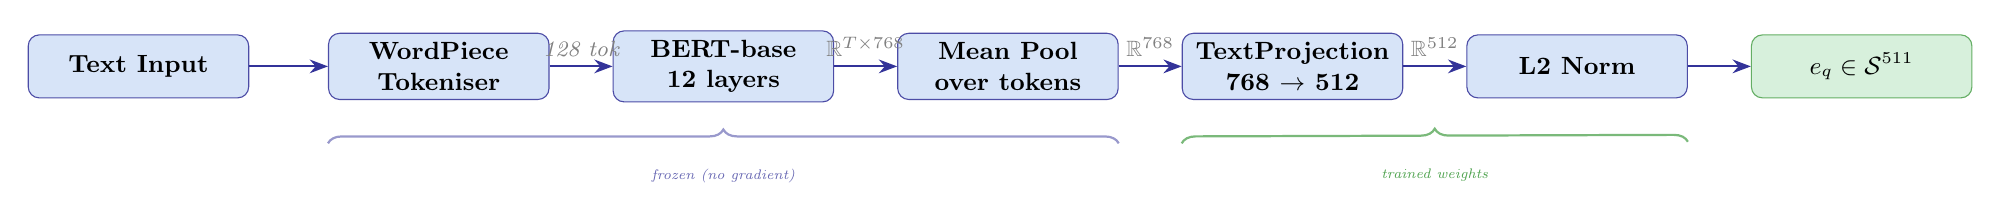
\begin{tikzpicture}[
  node distance=0.5cm and 0.8cm,
  block/.style={rectangle, rounded corners=4pt, draw=NavyBlue!70,
    fill=bluebox, minimum width=2.8cm, minimum height=0.8cm,
    font=\small\bfseries, align=center},
  arr/.style={->, >=Stealth, thick, NavyBlue!80},
  dimlabel/.style={font=\footnotesize\itshape, text=gray}
]
  \node[block] (input)  {Text Input};
  \node[block, right=1.0cm of input]  (tok)   {WordPiece\\Tokeniser};
  \node[block, right=0.8cm of tok]    (bert)  {BERT-base\\12 layers};
  \node[block, right=0.8cm of bert]   (pool)  {Mean Pool\\over tokens};
  \node[block, right=0.8cm of pool]   (proj)  {TextProjection\\768 $\to$ 512};
  \node[block, right=0.8cm of proj]   (norm)  {L2 Norm};
  \node[block, right=0.8cm of norm, fill=greenbox, draw=ForestGreen!70]   (out)   {$e_q \in \mathcal{S}^{511}$};

  \draw[arr] (input) -- (tok);
  \draw[arr] (tok)   -- node[above,dimlabel]{128 tok} (bert);
  \draw[arr] (bert)  -- node[above,dimlabel]{$\mathbb{R}^{T\times768}$} (pool);
  \draw[arr] (pool)  -- node[above,dimlabel]{$\mathbb{R}^{768}$} (proj);
  \draw[arr] (proj)  -- node[above,dimlabel]{$\mathbb{R}^{512}$} (norm);
  \draw[arr] (norm)  -- (out);

  %% freeze indicator
  \draw[decorate, decoration={brace,amplitude=5pt}, NavyBlue!40, thick]
    ([yshift=-0.55cm]tok.south west) -- ([yshift=-0.55cm]pool.south east)
    node[midway, below=0.2cm, font=\tiny\itshape, text=NavyBlue!60]{frozen (no gradient)};

  \draw[decorate, decoration={brace,amplitude=5pt}, ForestGreen!60, thick]
    ([yshift=-0.55cm]proj.south west) -- ([yshift=-0.55cm]norm.south east)
    node[midway, below=0.2cm, font=\tiny\itshape, text=ForestGreen!80]{trained weights};
\end{tikzpicture}
\caption{TextEncoderV2 architecture. BERT backbone is frozen; only TextProjection is trained.}
\end{figure}

\subsubsection{Step-by-Step Algorithm}

\begin{algorithm}[H]
\caption{TextEncoderV2.encode($\text{text}$)}
\label{alg:textencode}
\begin{algorithmic}[1]
\Require text $t \in$ String, frozen BERT, trained TextProjection $P_\theta$
\Ensure $e_q \in \Sph^{511}$, entities $\mathcal{E}_q$, domain\_hint
\State \textbf{// Step 1: Tokenise with WordPiece (max 128 tokens)}
\State $\text{tokens} \gets \text{tokeniser}(t,\; \texttt{max\_length}=128,\; \texttt{truncation}=\text{True})$
\State \textbf{// Step 2: BERT forward pass — no gradient (frozen)}
\State $H \gets \text{BERT}(\text{tokens})\texttt{.last\_hidden\_state}$ \Comment{shape: $(1, T, 768)$}
\State $h_{\text{BERT}} \gets \frac{1}{T}\sum_{t=1}^T H_{t}$ \Comment{mean pool: $(1, 768)$}
\State \textbf{// Step 3: TextProjection — trainable}
\State $e_{\text{raw}} \gets P_\theta(h_{\text{BERT}})$ \Comment{$768 \to 512$}
\State $e_q \gets e_{\text{raw}} / \|e_{\text{raw}}\|_2$ \Comment{L2 normalise onto $\Sph^{511}$}
\State \textbf{// Step 4: NER entity extraction (spaCy)}
\State $\mathcal{E}_q \gets \{\text{noun\_chunks}\} \cup \{\text{named\_entities}\}$ (lowercased, deduplicated)
\State \textbf{// Step 5: Domain keyword counting}
\State $n_m \gets |\{w \in \text{MEDICAL\_TERMS} : w \subseteq t.\text{lower}()\}|$
\State $\text{domain\_hint} \gets$ ``\texttt{medical}'' if $n_m \ge 2$ else \texttt{None}
\State \Return $(e_q,\; \mathcal{E}_q,\; \text{domain\_hint})$
\end{algorithmic}
\end{algorithm}

\subsubsection{TextProjection Network}

\begin{definition}[TextProjection]
$\text{TextProjection} : \R^{768} \to \Sph^{511}$ is defined as:
\[
  h_1 = W_1 x + b_1 \in \R^{768} \quad\text{(Linear, proj.0)}
\]
\[
  h_2 = \GELU(h_1) \quad\text{(activation)}
\]
\[
  h_3 = \LN(h_2) \in \R^{768} \quad\text{(LayerNorm, proj.2)}
\]
\[
  h_4 = W_2 h_3 + b_2 \in \R^{512} \quad\text{(Linear, proj.3)}
\]
\[
  h_5 = \LN(h_4) \in \R^{512} \quad\text{(LayerNorm, norm)}
\]
\[
  \hat{e} = h_5 / \|h_5\|_2 \in \Sph^{511} \quad\text{(L2 normalise)}
\]
\end{definition}

\begin{remark}[Mean Pooling vs.\ CLS Token]
BERT's \texttt{[CLS]} token: $e = H_{:,0,:}$ — optimised for classification but
degrades for long sequences. Mean pooling: $e = \frac{1}{T}\sum_{t=1}^T H_{:,t,:}$
— averages all token representations, better for semantic similarity and information
retrieval tasks (consistent with sentence-transformers literature).
\end{remark}

\begin{tcolorbox}[laymanbox]
BERT reads the question and produces 768 numbers for each word.
We average all those numbers to get one 768-number ``meaning vector'' for the
whole sentence. Then TextProjection squeezes it from 768 down to 512 numbers while
preserving the meaning — like compressing a file without losing important content.
Finally, we scale it to length exactly 1, so all queries live on the same ``ball''.
\end{tcolorbox}

\subsection{AudioEncoderV2: Wav2Vec + Whisper + Emotion Classification}

\subsubsection{Two-Stream Processing}

\begin{figure}[htbp]
\centering
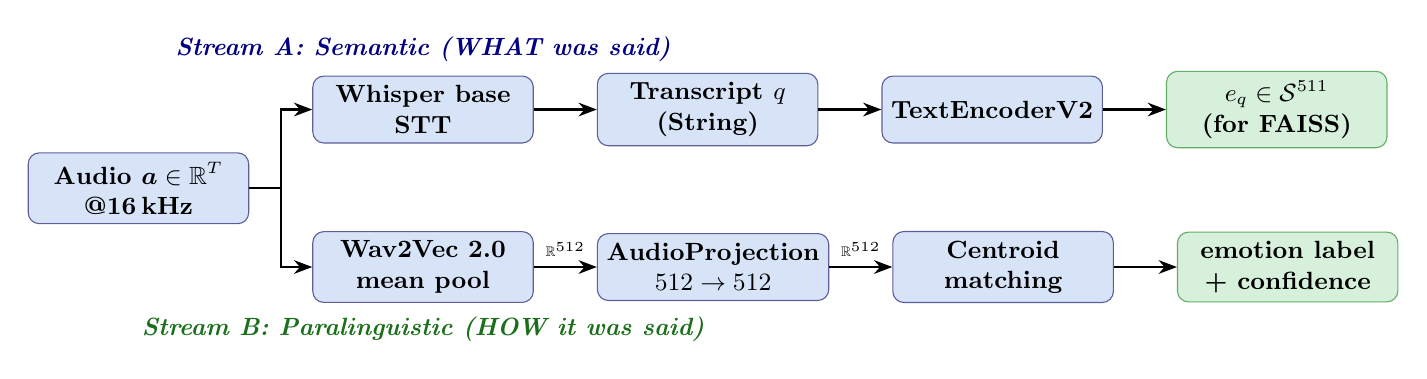
\begin{tikzpicture}[
  node distance=0.5cm and 0.7cm,
  block/.style={rectangle, rounded corners=4pt, draw=MidnightBlue!70,
    fill=bluebox, minimum width=2.8cm, minimum height=0.85cm,
    font=\small\bfseries, align=center},
  block2/.style={rectangle, rounded corners=4pt, draw=ForestGreen!70,
    fill=greenbox, minimum width=2.8cm, minimum height=0.85cm,
    font=\small\bfseries, align=center},
  arr/.style={->, >=Stealth, thick}
]
  \node[block] (audio) {Audio $\bm{a} \in \mathbb{R}^T$\\@16\,kHz};

  %% Stream A
  \node[block, right=0.8cm of audio, yshift=1.0cm] (whisper)
    {Whisper base\\STT};
  \node[block, right=0.8cm of whisper] (trans)
    {Transcript $q$\\(String)};
  \node[block, right=0.8cm of trans] (textenc)
    {TextEncoderV2};
  \node[block2, right=0.8cm of textenc] (textemb)
    {$e_q \in \Sph^{511}$\\(for FAISS)};

  %% Stream B
  \node[block, right=0.8cm of audio, yshift=-1.0cm] (wav2vec)
    {Wav2Vec 2.0\\mean pool};
  \node[block, right=0.8cm of wav2vec] (audioproj)
    {AudioProjection\\$512\to512$};
  \node[block, right=0.8cm of audioproj] (emotion)
    {Centroid\\matching};
  \node[block2, right=0.8cm of emotion] (emoout)
    {emotion label\\+ confidence};

  \draw[->, >=Stealth, thick] (audio.east) -- ++(0.4,0) |- (whisper.west);
  \draw[->, >=Stealth, thick] (audio.east) -- ++(0.4,0) |- (wav2vec.west);
  \draw[->, >=Stealth, thick] (whisper) -- (trans);
  \draw[->, >=Stealth, thick] (trans) -- (textenc);
  \draw[->, >=Stealth, thick] (textenc) -- (textemb);
  \draw[->, >=Stealth, thick] (wav2vec) -- node[above,font=\tiny]{$\mathbb{R}^{512}$} (audioproj);
  \draw[->, >=Stealth, thick] (audioproj) -- node[above,font=\tiny]{$\mathbb{R}^{512}$} (emotion);
  \draw[->, >=Stealth, thick] (emotion) -- (emoout);

  \node[font=\small\bfseries\itshape, text=NavyBlue, above=0.05cm of whisper]
    {Stream A: Semantic (WHAT was said)};
  \node[font=\small\bfseries\itshape, text=ForestGreen!80!black, below=0.05cm of wav2vec]
    {Stream B: Paralinguistic (HOW it was said)};
\end{tikzpicture}
\caption{AudioEncoderV2 dual-stream architecture. Stream A produces the query
embedding used for retrieval; Stream B produces the emotion label used to modulate
the LLM system prompt.}
\end{figure}

\subsubsection{Emotion Centroid Matching Algorithm}

\begin{definition}[Emotion Centroids]
Given RAVDESS training embeddings $\{(f_i, \ell_i)\}$ where $f_i \in \R^{512}$
and $\ell_i \in \mathcal{C} = \{\text{angry, calm, disgust, fearful, happy, neutral, sad, surprised}\}$:
\[
  \mu_c = \frac{1}{|S_c|}\sum_{f \in S_c} \text{AudioProjection}(f), \qquad
  S_c = \{f_i : \ell_i = c\}
\]
\[
  C_c = \frac{\mu_c}{\|\mu_c\|_2} \in \Sph^{511}, \quad c \in \mathcal{C}.
\]
The centroids matrix is $\mathbf{C} \in \R^{8 \times 512}$.
\end{definition}

\begin{algorithm}[H]
\caption{Emotion Classification via Centroid Matching}
\label{alg:emotion}
\begin{algorithmic}[1]
\Require audio embedding $e_{\text{audio}} \in \Sph^{511}$, centroids $\mathbf{C} \in \R^{8\times512}$
\Ensure emotion label, confidence $\in [-1,1]$
\State $\bm{s} \gets \mathbf{C} \cdot e_{\text{audio}}^\top$
  \Comment{$s_i = C_i \cdot e_{\text{audio}}$ (cosine sim, by Lemma~\ref{lem:cosdot})}
\State $i^* \gets \argmax_{i} s_i$
\State $\text{emotion} \gets \mathcal{C}[i^*]$
\State $\text{confidence} \gets s_{i^*}$
\State \Return $(\text{emotion},\; \text{confidence})$
\end{algorithmic}
\end{algorithm}

\begin{remark}[Prototype Learning]
This is a form of class prototype learning (Snell et al., 2017 — Prototypical Networks).
The centroid $C_c$ represents the ``average sound'' of emotion $c$ in the shared
embedding space. At inference, one forward pass through AudioProjection and one
matrix multiply is sufficient — no separate classification head required.
\end{remark}

\subsection{MultiModalFusion Transformer}

\begin{definition}[Multi-Modal Fusion]
Given modality embeddings $e_t \in \R^{768}$, $e_i \in \R^{768}$,
$e_v \in \R^{512}$, $e_s \in \R^{256}$, the fusion network:
\[
  \mathbf{T} = \begin{bmatrix}
    W_t e_t \\ W_i e_i \\ W_v e_v \\ W_s e_s
  \end{bmatrix} \in \R^{4 \times 512}, \quad
  \tilde{\mathbf{T}} = \LN(\mathbf{T})
\]
\[
  \mathbf{F},\; \text{attn} = \MHA(\tilde{\mathbf{T}}, \tilde{\mathbf{T}}, \tilde{\mathbf{T}})
\]
\[
  \mathbf{H} = \LN(\mathbf{F} + \tilde{\mathbf{T}}), \qquad
  \mathbf{H}' = \LN\!\left(\mathbf{H} + \mathrm{FFN}(\mathbf{H})\right)
\]
\[
  e_{\text{fused}} = W_o \cdot \frac{1}{4}\sum_{m=1}^{4} H'_m \in \R^{512}
\]
\end{definition}

\begin{axiom}[Missing-Modality Robustness]
A zero vector $\bm{0} \in \R^d$ projected through a linear layer $W\bm{0} = \bm{0}$.
Therefore, absent modalities (voice, sensor) at inference time contribute a zero token
to the attention sequence without injecting noise. The model gracefully degrades to
text-only mode when only text is provided.
\end{axiom}

%%
%% ============================================================
%% SECTION 5 — KNOWLEDGE GRAPH
%% ============================================================
%%
\newpage
\section{Knowledge Graph Construction}

\begin{definition}[Knowledge Graph]
\[
  \KG = (\mathcal{V},\; \Ent,\; \mathcal{R})
\]
where $\mathcal{V}$ is the set of entity nodes (top-100 frequent non-stopword tokens),
$\Ent \subseteq \mathcal{V} \times \mathcal{R} \times \mathcal{V}$ is the set of typed edges,
and $\mathcal{R} = \{\texttt{appears\_with}\}$ is the relation type set.
\end{definition}

\begin{algorithm}[H]
\caption{KG Construction from Captions}
\label{alg:kg}
\begin{algorithmic}[1]
\Require Dataset $\mathcal{D} = \{t_1, \ldots, t_n\}$, stopwords $\mathcal{S}$,
         $\texttt{top\_entities}=100$
\Ensure Knowledge graph $\KG$
\State $\text{all\_words} \gets []$
\ForEach{$t_i \in \mathcal{D}$}
  \State $\text{all\_words} \mathrel{+}= \text{regex\_words}(t_i.\text{lower}())$
\EndFor
\State $\text{counts} \gets \text{Counter}(\text{all\_words})$
\State $\mathcal{V} \gets \text{top-100 words not in } \mathcal{S} \text{ with } |\text{word}| > 3$
\State $\KG \gets \text{empty}$
\ForEach{$(v, \text{freq}) \in \mathcal{V}$}
  \State $\KG.\text{add\_entity}(v)$
\EndFor
\ForEach{$t_i \in \mathcal{D}_{:3000}$}
  \State $E_i \gets \{v \in \mathcal{V} : v \in t_i\}$ \Comment{entities in this caption}
  \ForEach{$e_1, e_2 \in E_i$ with $e_1 \ne e_2$}
    \State $\KG.\text{add\_relationship}(e_1, \texttt{appears\_with}, e_2)$
  \EndFor
\EndFor
\State \Return $\KG$
\end{algorithmic}
\end{algorithm}

\begin{algorithm}[H]
\caption{KG Depth-First Neighbour Search}
\label{alg:kgdfs}
\begin{algorithmic}[1]
\Require entity $v$, $\KG$, max\_hops $= 2$
\Ensure neighbours list
\State $\text{visited} \gets \emptyset$; $\text{neighbours} \gets []$
\State \Call{DFS}{$v$, 1}
\Procedure{DFS}{$\text{current}$, $\text{hops}$}
  \If{$\text{hops} > \text{max\_hops}$ \textbf{or} $\text{current} \in \text{visited}$}
    \State \Return
  \EndIf
  \State $\text{visited} \gets \text{visited} \cup \{\text{current}\}$
  \ForEach{$(h, r, t) \in \KG.\text{relationships}$}
    \If{$h = \text{current}$}
      \State $\text{neighbours}.\text{append}(h, r, t, \text{hops})$; \Call{DFS}{$t$, $\text{hops}+1$}
    \ElsIf{$t = \text{current}$}
      \State $\text{neighbours}.\text{append}(t, r\_\text{inv}, h, \text{hops})$; \Call{DFS}{$h$, $\text{hops}+1$}
    \EndIf
  \EndFor
\EndProcedure
\end{algorithmic}
\end{algorithm}

%%
%% ============================================================
%% SECTION 6 — CONTRASTIVE LEARNING
%% ============================================================
%%
\newpage
\section{Contrastive Learning: InfoNCE Loss}

\subsection{Why Not MSE?}

The original (buggy) version used Mean Squared Error:
\[
  \Loss_{\text{MSE}} = \frac{1}{d}\|e_{\text{fused}} - e_{\text{text}}\|_2^2.
\]
This fails because:
\begin{enumerate}
  \item It ignores the relative positions of all \emph{other} examples in the batch.
  \item It can be trivially minimised by \textbf{representation collapse}: setting all embeddings to $\bm{0}$.
  \item MSE $\approx 0.0008$ was observed in training — an impossibly small value indicating collapse, not good learning.
\end{enumerate}

\subsection{InfoNCE Contrastive Loss}

\begin{definition}[InfoNCE Loss]
Given a batch of $B$ positive pairs $\{(e_i^{(1)}, e_i^{(2)})\}_{i=1}^B$ where
$e^{(1)}$ are fused embeddings and $e^{(2)}$ are text-projected embeddings:
\[
  S_{ij} = \hat{e}_i^{(1)} \cdot \hat{e}_j^{(2)}, \qquad
  \hat{e} = e/\|e\|_2
\]
\[
  \boxed{\Loss_{\text{InfoNCE}} = -\frac{1}{B}\sum_{i=1}^B
    \log\frac{\exp(S_{ii}/\tau)}{\sum_{j=1}^B \exp(S_{ij}/\tau)}}
\]
where $\tau = 0.07$ is the temperature hyperparameter.
\end{definition}

\begin{theorem}[InfoNCE as Cross-Entropy]
The InfoNCE loss is equivalent to cross-entropy loss over a $B$-way classification
problem where the target label for row $i$ is the diagonal index $i$:
\[
  \Loss_{\text{InfoNCE}} = \frac{1}{B}\sum_{i=1}^B
    \mathrm{CE}\!\left(\frac{S_{i,:}}{\tau},\; i\right).
\]
The \textbf{symmetric} version (used in code) averages both directions:
\[
  \Loss_{\text{sym}} = \frac{1}{2}\left[
    \mathrm{CE}\!\left(\frac{S}{\tau},\; \bm{y}\right) +
    \mathrm{CE}\!\left(\frac{S^\top}{\tau},\; \bm{y}\right)
  \right], \quad \bm{y} = [0, 1, \ldots, B{-}1].
\]
\end{theorem}

\begin{lemma}[Random Baseline Loss]
For a randomly initialised model with $B$ examples per batch:
\[
  \mathbb{E}[\Loss_{\text{InfoNCE}}]_{\text{random}} = \log B.
\]
For $B = 32$: $\log 32 \approx 3.47$.
\end{lemma}
\begin{proof}
At initialisation, $S_{ij}$ are near-uniform due to random embeddings.
The softmax denominator $\sum_j \exp(S_{ij}/\tau) \approx B \cdot \exp(S_{ii}/\tau)$,
giving $-\log(1/B) = \log B$.
\end{proof}

\begin{tcolorbox}[keybox, title=Training Convergence Diagnostic]
\begin{tabular}{lll}
\toprule
Observation & Interpretation & Action \\
\midrule
Loss $\approx \log B$ at start & Normal random init & Continue \\
Loss $\to$ 0.3--0.8 after 10 epochs & \textbf{Healthy convergence} & \\
Loss $< 0.05$ at any epoch & Representation collapse & Stop, debug \\
Loss $\approx 0.0008$ & MSE collapse (old bug) & Switch to InfoNCE \\
\bottomrule
\end{tabular}
\end{tcolorbox}

\begin{tcolorbox}[laymanbox]
InfoNCE loss works like a matching game. In each batch of 32 pairs (image+caption),
the model must correctly identify which caption goes with which image. The loss
measures how well it does: a score of 3.47 (= log 32) means pure guessing;
a score of 0.5 means the model is correctly matching most pairs.
Importantly, it compares EACH item against ALL others in the batch —
making it much harder to cheat by just outputting zero for everything.
\end{tcolorbox}

\subsection{Temperature Parameter}

\begin{definition}[Temperature $\tau$]
The temperature $\tau > 0$ controls the sharpness of the softmax distribution:
\begin{itemize}
  \item $\tau \to 0$: hard selection (greedy), very sharp distribution
  \item $\tau = 1$: standard softmax
  \item $\tau \to \infty$: uniform distribution (no discrimination)
\end{itemize}
CLIP paper recommendation: $\tau = 0.07$. Rationale: low temperature forces the
model to be more discriminative, pushing positive pairs close together and
negative pairs far apart on $\Sph^{511}$.
\end{definition}

%%
%% ============================================================
%% SECTION 7 — OPTIMISATION
%% ============================================================
%%
\newpage
\section{Optimisation: AdamW and Cosine Scheduler}

\subsection{AdamW Update Rule}

\begin{definition}[AdamW]
Given gradient $g_t = \nabla_\theta \Loss_t$, the AdamW update is:
\[
  m_t = \beta_1 m_{t-1} + (1-\beta_1) g_t, \qquad v_t = \beta_2 v_{t-1} + (1-\beta_2)g_t^2
\]
\[
  \hat{m}_t = \frac{m_t}{1-\beta_1^t}, \qquad \hat{v}_t = \frac{v_t}{1-\beta_2^t}
\]
\[
  \boxed{\theta_{t+1} = \theta_t - \eta \cdot \frac{\hat{m}_t}{\sqrt{\hat{v}_t}+\varepsilon} - \eta\lambda\theta_t}
\]
where $\eta = 10^{-4}$ (learning rate), $\lambda = 0.01$ (decoupled weight decay),
$\beta_1 = 0.9$, $\beta_2 = 0.999$, $\varepsilon = 10^{-8}$.
\end{definition}

\begin{remark}[Decoupled Weight Decay]
The last term $\eta\lambda\theta_t$ is the \textbf{decoupled} weight decay.
In standard Adam, weight decay is applied inside the adaptive scaling (incorrect);
AdamW applies it directly to parameters, giving $\ell_2$ regularisation with the
correct effective regularisation strength regardless of gradient magnitude.
\end{remark}

\subsection{Cosine Annealing Scheduler}

\[
  \eta_t = \eta_{\min} + \frac{1}{2}(\eta_{\max} - \eta_{\min})\left(1 + \cos\!\frac{t\pi}{T}\right)
\]
where $T = |\text{loader}| \times E$ is the total number of steps
($= 157 \times 10 = 1570$ for 5K images, batch 32, 10 epochs).

\begin{tcolorbox}[laymanbox]
AdamW is the ``smart gradient descent'' used to train the model.
Instead of taking equal steps in all directions, it adapts the step size
separately for each weight: large steps for rarely-updated weights,
small steps for frequently-updated weights. The cosine scheduler gradually
reduces the learning rate during training — like easing your foot off the
accelerator as you approach a parking spot — so the model settles into a
good solution rather than overshooting.
\end{tcolorbox}

\subsection{Training Loop Algorithm}

\begin{algorithm}[H]
\caption{Single Training Epoch (train\_epoch)}
\label{alg:trainepoch}
\begin{algorithmic}[1]
\Require Fusion $F$, ImageEncoder $E$, Projection $P$, Retriever $R$,
         DataLoader $L$, optimizer, $\tau = 0.07$
\Ensure Updated weights $F, E, P$; per-epoch average loss
\State $\text{total\_loss} \gets 0$
\ForEach{batch $(I \in \R^{B\times3\times224\times224},\; T) \in L$}
  \State \textbf{// \textcircled{1} Frozen BERT encoding (no gradient)}
  \State $e_t^{(b)} \gets R.\text{encode}(T[b])$ for $b=1\ldots B$ $\Rightarrow E_T \in \R^{B\times768}$
  \State \textbf{// \textcircled{2} Image encoding (trainable projection)}
  \State $E_I \gets E(I) \in \R^{B\times768}$
  \State \textbf{// \textcircled{3} Zero-pad absent modalities}
  \State $E_V \gets \bm{0}^{B\times512}$; $E_S \gets \bm{0}^{B\times256}$
  \State \textbf{// \textcircled{4} Multi-modal fusion}
  \State $e_{\text{fused}},\; \text{attn} \gets F(E_T, E_I, E_V, E_S) \in \R^{B\times512}$
  \State \textbf{// \textcircled{5} Project text to comparison space}
  \State $e_{\text{proj}} \gets P(E_T) \in \R^{B\times512}$
  \State \textbf{// \textcircled{6} Symmetric InfoNCE loss}
  \State $\Loss \gets \Loss_{\text{InfoNCE}}(e_{\text{fused}},\; e_{\text{proj}},\; \tau)$
  \State \textbf{// \textcircled{7} Backward pass}
  \State optimizer.zero\_grad()
  \State $\Loss.\text{backward}()$
  \State $\text{clip\_grad\_norm}(\nabla\theta,\; \text{max}=1.0)$ \Comment{prevent exploding gradients}
  \State optimizer.step(); scheduler.step()
  \State $\text{total\_loss} \mathrel{+}= \Loss.\text{item}()$
\EndFor
\State \Return $\text{total\_loss} / |L|$
\end{algorithmic}
\end{algorithm}

\begin{remark}[Gradient Clipping]
Gradient clipping: $g \gets g \cdot \min\!\left(1,\; \frac{1}{\|g\|_2}\right)$
ensures $\|g\|_2 \le 1.0$. Prevents exploding gradients, which is especially
important during early training when the model is far from convergence.
\end{remark}

%%
%% ============================================================
%% SECTION 8 — RETRIEVAL ENGINE
%% ============================================================
%%
\newpage
\section{Two-Stage Hybrid Retrieval (Phase 2)}

\subsection{Retrieval Architecture Overview}

\begin{figure}[htbp]
\centering
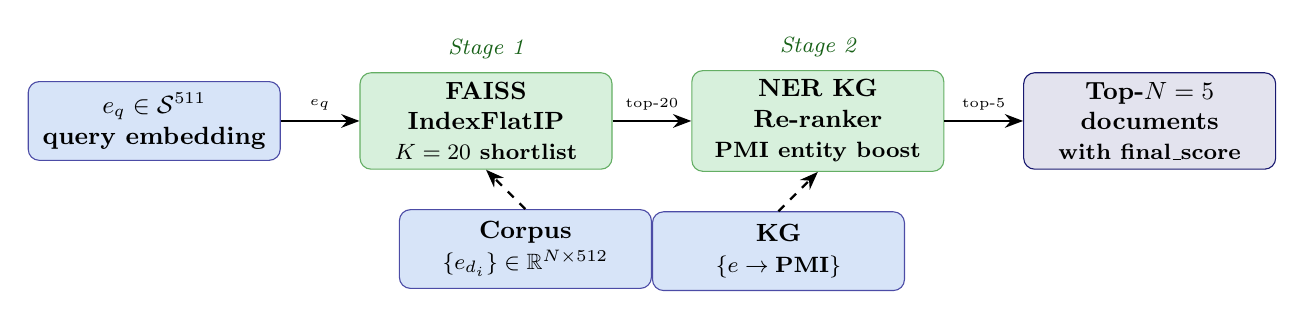
\begin{tikzpicture}[
  node distance=0.6cm and 0.9cm,
  block/.style={rectangle, rounded corners=4pt, draw=ForestGreen!70,
    fill=greenbox, minimum width=3.2cm, minimum height=1.0cm,
    font=\small\bfseries, align=center},
  block2/.style={rectangle, rounded corners=4pt, draw=NavyBlue!70,
    fill=bluebox, minimum width=3.2cm, minimum height=1.0cm,
    font=\small\bfseries, align=center},
  outnod/.style={rectangle, rounded corners=4pt, draw=MidnightBlue,
    fill=MidnightBlue!12, minimum width=3.2cm, minimum height=1.0cm,
    font=\small\bfseries, align=center},
  arr/.style={->, >=Stealth, thick}
]
  \node[block2] (qemb)   {$e_q \in \Sph^{511}$\\query embedding};
  \node[block,  right=1.0cm of qemb]  (faiss)
    {FAISS\\IndexFlatIP\\\footnotesize$K=20$ shortlist};
  \node[block,  right=1.0cm of faiss] (kgrank)
    {NER KG\\Re-ranker\\\footnotesize PMI entity boost};
  \node[outnod, right=1.0cm of kgrank](topn)
    {Top-$N=5$\\documents\\\footnotesize with final\_score};

  \node[block2, below=0.5cm of faiss, xshift=0.5cm] (corpus)
    {Corpus\\\footnotesize $\{e_{d_i}\} \in \R^{N\times512}$};
  \node[block2, below=0.5cm of kgrank, xshift=-0.5cm] (kg)
    {KG\\\footnotesize $\{e \to \text{PMI}\}$};

  \draw[arr] (qemb) -- node[above,font=\tiny]{$e_q$} (faiss);
  \draw[arr] (faiss) -- node[above,font=\tiny]{top-20} (kgrank);
  \draw[arr] (kgrank) -- node[above,font=\tiny]{top-5} (topn);
  \draw[arr, dashed] (corpus.north) -- (faiss.south);
  \draw[arr, dashed] (kg.north) -- (kgrank.south);

  \node[font=\footnotesize\itshape, text=ForestGreen!70!black,
    above=0.05cm of faiss]{Stage 1};
  \node[font=\footnotesize\itshape, text=ForestGreen!70!black,
    above=0.05cm of kgrank]{Stage 2};
\end{tikzpicture}
\caption{Two-stage hybrid retrieval. Stage 1 uses FAISS for approximate nearest
neighbour search; Stage 2 uses knowledge graph entity re-ranking within the shortlist.}
\end{figure}

\subsection{Stage 1: FAISS Dense Retrieval}

\begin{definition}[FAISS IndexFlatIP Search]
Let $\mathcal{C} = \{e_{d_1},\ldots,e_{d_N}\} \subset \Sph^{511}$ be the corpus embeddings.
Given query $e_q \in \Sph^{511}$:
\[
  \text{dense\_score}(q, d_i) = e_q \cdot e_{d_i} \in [-1, 1]
\]
\[
  \mathcal{R}_K = \argtopk_{i \in 1\ldots N}\; (e_q \cdot e_{d_i})
\]
\end{definition}

\begin{proposition}[FAISS Complexity]
FAISS IndexFlatIP (exact, brute-force) has per-query complexity:
\[
  O(N \cdot d) = O(69{,}866 \times 512) \approx 3.58 \times 10^7 \text{ multiply-adds}.
\]
On GPU: $\approx 1\,\text{ms}$. On CPU: $\approx 15\,\text{ms}$.
\end{proposition}

\subsection{Stage 2: KG Entity Re-ranking}

\subsubsection{Pointwise Mutual Information (PMI)}

\begin{definition}[PMI]
For entities $a, b$ in a corpus:
\[
  \mathrm{PMI}(a, b) = \log\frac{P(a,b)}{P(a)\,P(b)}
\]
where $P(a,b)$ is the probability of co-occurrence in a document and
$P(a), P(b)$ are marginal probabilities. $\mathrm{PMI} > 0$ indicates
$a$ and $b$ co-occur more than chance.
\end{definition}

\subsubsection{Full Re-ranking Algorithm}

\begin{algorithm}[H]
\caption{NERKGReranker.rerank}
\label{alg:rerank}
\begin{algorithmic}[1]
\Require Shortlist $S = [d_1, \ldots, d_K]$ with dense\_score, query\_entities $\mathcal{E}_q$,
         KG, top\_n $N$, $\alpha = 0.7$
\Ensure Top-$N$ documents with final\_score
\State \textbf{// Step 1: Min-max normalise dense scores within shortlist}
\State $s_{\min} \gets \min_i \text{dense\_score}(d_i)$;
       $s_{\max} \gets \max_i \text{dense\_score}(d_i)$
\State $\Delta \gets s_{\max} - s_{\min}$ (set to 1 if $\Delta = 0$)
\State $\tilde{s}_{\text{dense}}(d_i) \gets (\text{dense\_score}(d_i) - s_{\min}) / \Delta \in [0,1]$
\State \textbf{// Step 2: Compute PMI-weighted entity overlap scores}
\ForEach{$d_i \in S$}
  \State $\mathcal{E}_{d_i} \gets \text{entity\_extract}(d_i.\text{text})$
    \Comment{word-boundary regex}
  \State $\text{kg\_raw}(d_i) \gets
    \sum_{q \in \mathcal{E}_q}\sum_{d \in \mathcal{E}_{d_i}}
    \mathrm{PMI}(q, d) \cdot \mathbf{1}[q \in \mathrm{KG},\; d \in \mathrm{KG}[q]]$
\EndFor
\State \textbf{// Step 3: Normalise KG scores}
\State $m_\mathrm{KG} \gets \max_i \text{kg\_raw}(d_i)$ (set to 1 if $= 0$)
\State $\tilde{s}_{\text{KG}}(d_i) \gets \text{kg\_raw}(d_i) / m_\mathrm{KG} \in [0,1]$
\State \textbf{// Step 4: Combine}
\ForEach{$d_i \in S$}
  \State $\text{final\_score}(d_i) \gets
    \alpha \cdot \tilde{s}_{\text{dense}}(d_i) + (1-\alpha)\cdot\tilde{s}_{\text{KG}}(d_i)$
\EndFor
\State \textbf{// Step 5: Sort and truncate}
\State \Return $\mathrm{top\text{-}N}\!\left(S,\; \text{by final\_score desc}\right)$
\end{algorithmic}
\end{algorithm}

\begin{theorem}[Score Bounds]
Under Algorithm~\ref{alg:rerank}, all final scores satisfy:
\[
  \text{final\_score}(d_i) \in [0, 1] \quad \forall d_i \in S.
\]
\end{theorem}
\begin{proof}
By construction: $\tilde{s}_{\text{dense}} \in [0,1]$ (min-max normalisation),
$\tilde{s}_{\text{KG}} \in [0,1]$ (division by maximum).
Since $\alpha \in (0,1)$ and $\alpha + (1-\alpha) = 1$:
$\text{final\_score} = \alpha\cdot[0,1] + (1-\alpha)\cdot[0,1] \in [0,1]$.
\end{proof}

\begin{remark}[Word-Boundary Regex]
Entity matching uses \texttt{r'\textbackslash b\{entity\}\textbackslash b'} to prevent
substring false positives: \texttt{``cat''} matches \texttt{``cat''} but not
\texttt{``category''}, \texttt{``scatter''}, or \texttt{``catfish''}. Critical for
medical domain where \texttt{``mass''} $\ne$ \texttt{``massive''} and
\texttt{``pleural''} $\ne$ \texttt{``plural''}.
\end{remark}

\subsection{Hybrid Retriever (FusionRetriever)}

\begin{definition}[Hybrid Score]
For the Month 1 retriever, the hybrid score combines dense and graph boost:
\[
  \text{hybrid}(q, d) = \alpha \cdot \text{dense}(q,d) + (1-\alpha)\cdot\text{boost}(q,d)
\]
where $\alpha = 0.6$,
\[
  \text{boost}(q, d) = \min\!\left(1,\; \max_{e \in \mathcal{E}_q}\max_{(e, r, n, h) \in \mathrm{KG}} \frac{\mathbf{1}[n \in d]}{h+1}\right)
\]
and $h$ is the hop count in the KG. Closer neighbours (smaller $h$) produce higher boosts.
\end{definition}

%%
%% ============================================================
%% SECTION 9 — GENERATION WITH TIERED CONFIDENCE
%% ============================================================
%%
\newpage
\section{Generation Layer with Tiered Confidence (Phase 3)}

\subsection{Tiered Confidence System}

\begin{definition}[Confidence Tier Function]
Given max retrieval score $s$ and domain threshold $\tau$:
\[
  \mathrm{tier}(s) = \begin{cases}
    \texttt{full}     & \text{if } s \ge \tau \\
    \texttt{partial}  & \text{if } \tau - 0.2 \le s < \tau \\
    \texttt{rejected} & \text{if } s < \tau - 0.2
  \end{cases}
\]
\end{definition}

\begin{figure}[htbp]
\centering
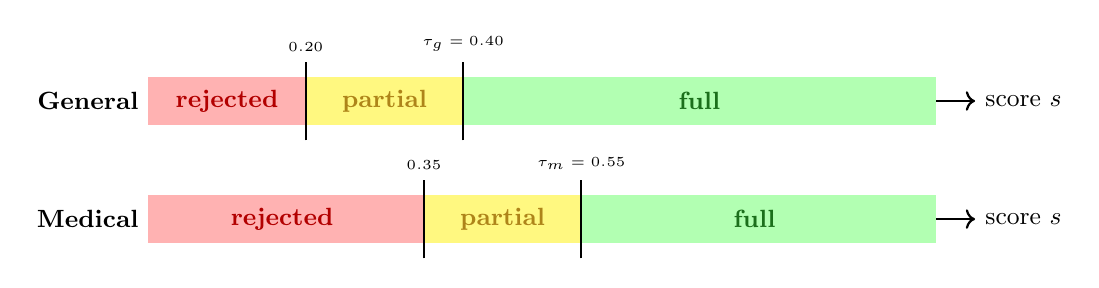
\begin{tikzpicture}[scale=1.0]
  %% General domain axis
  \draw[thick, ->] (0,1.5) -- (10.5, 1.5) node[right]{\small score $s$};
  \node[left, font=\small\bfseries] at (0,1.5) {General};

  \fill[red!30]    (0,1.2) rectangle (2, 1.8);
  \fill[yellow!50] (2,1.2) rectangle (4, 1.8);
  \fill[green!30]  (4,1.2) rectangle (10,1.8);

  \draw[thick] (2,1.0) -- (2,2.0) node[above,font=\tiny]{$0.20$};
  \draw[thick] (4,1.0) -- (4,2.0) node[above,font=\tiny]{$\tau_g=0.40$};

  \node[font=\small, red!70!black]   at (1,1.5) {\textbf{rejected}};
  \node[font=\small, Goldenrod!80!black] at (3,1.5) {\textbf{partial}};
  \node[font=\small, ForestGreen!80!black] at (7,1.5) {\textbf{full}};

  %% Medical domain axis
  \draw[thick, ->] (0,0) -- (10.5, 0) node[right]{\small score $s$};
  \node[left, font=\small\bfseries] at (0,0) {Medical};

  \fill[red!30]    (0,-0.3) rectangle (3.5,0.3);
  \fill[yellow!50] (3.5,-0.3) rectangle (5.5, 0.3);
  \fill[green!30]  (5.5,-0.3) rectangle (10, 0.3);

  \draw[thick] (3.5,-0.5) -- (3.5,0.5) node[above,font=\tiny]{$0.35$};
  \draw[thick] (5.5,-0.5) -- (5.5,0.5) node[above,font=\tiny]{$\tau_m=0.55$};

  \node[font=\small, red!70!black]   at (1.7,0) {\textbf{rejected}};
  \node[font=\small, Goldenrod!80!black] at (4.5,0) {\textbf{partial}};
  \node[font=\small, ForestGreen!80!black] at (7.7,0) {\textbf{full}};
\end{tikzpicture}
\caption{Confidence tier partition for General ($\tau=0.40$) and Medical ($\tau=0.55$) domains.
The medical threshold is 0.15 higher, implementing the clinical safety constraint.}
\label{fig:tiers}
\end{figure}

\begin{axiom}[Clinical Safety Constraint]
For clinical domains, false positives (wrong answers stated confidently) carry
higher risk than false negatives (refusing to answer). Therefore:
\[
  \tau_{\text{medical}} = \tau_{\text{general}} + \Delta\tau_{\text{risk}} = 0.40 + 0.15 = 0.55.
\]
\end{axiom}

\subsection{Prompt Builder: 4-Section RAG Prompt}

\begin{definition}[RAG Prompt]
The structured prompt $\Pi_{\text{RAG}}$ has four sections:
\begin{enumerate}
  \item \textbf{Context block:} Retrieved documents with scores and image paths
  \item \textbf{Emotion modifier} (conditional, only if $\text{emotion\_conf} \ge 0.30$)
  \item \textbf{Uncertainty instruction} (only for \texttt{partial} tier)
  \item \textbf{Query + grounding instruction:} cite sources, no outside knowledge
\end{enumerate}
\end{definition}

\begin{tcolorbox}[keybox, title=Emotion Modifier Table]
\begin{tabular}{ll}
\toprule
Emotion & Modifier injected into system prompt \\
\midrule
angry    & ``Respond calmly and clearly'' \\
fearful  & ``Respond reassuringly'' \\
sad      & ``Respond with empathy'' \\
happy    & ``Match their energy'' \\
disgust  & ``Respond directly'' \\
surprised & ``Provide clear context'' \\
calm / neutral & (no modifier) \\
\bottomrule
\end{tabular}
\end{tcolorbox}

\begin{theorem}[RAG Faithfulness]
\label{thm:rag}
An answer is \textbf{faithful} to the retrieved context $\mathcal{D}^* = \{d_1,\ldots,d_N\}$
if and only if for every claim $c$ in the generated answer, there exists $d_j \in \mathcal{D}^*$
such that $c$ can be inferred from $d_j$. MIVA-KNIGHT enforces faithfulness by:
\begin{enumerate}
  \item Instructing the LLM: ``Answer using ONLY the retrieved context above''
  \item Requiring citation: ``Cite which Context number(s) support your answer''
  \item Rejecting low-confidence retrievals (tier = \texttt{rejected}) before any
    LLM call is made
\end{enumerate}
\end{theorem}

\begin{algorithm}[H]
\caption{Full Query Pipeline (MIVAKnight.query)}
\label{alg:query}
\begin{algorithmic}[1]
\Require user\_input: TextQuery or AudioQuery; loaded pipeline
\Ensure GeneratorOutput with answer, sources, emotion, audio (optional)
\State \textbf{// Phase 1: Encode input}
\If{user\_input is AudioQuery}
  \State $(\text{transcript}, \text{emotion}, \text{conf\_emo}, e_a) \gets \text{AudioEncoder.encode}(a)$
  \If{transcript $= \varnothing$}
    \State \Return rejection (empty transcript guard)
  \EndIf
  \State $(e_q, \mathcal{E}_q, h) \gets \text{TextEncoder.encode}(\text{transcript})$
\ElsIf{user\_input is TextQuery}
  \State $(e_q, \mathcal{E}_q, h) \gets \text{TextEncoder.encode}(q)$
  \State $\text{emotion} \gets$ ``neutral''; $\text{conf\_emo} \gets 0$
\EndIf
\State \textbf{// Phase 1b: Auto domain routing}
\If{$h \ne \varnothing$ \textbf{and} $h \ne \text{current domain}.\text{name}$}
  \State \Call{swap\_domain}{MedicalDomain() if $h=$ ``medical'' else GeneralDomain()}
\EndIf
\State \textbf{// Phase 2: Retrieval}
\State $(\mathcal{D}^*, s_{\max}, \text{passed}) \gets \text{HybridRetriever.retrieve}(e_q, \mathcal{E}_q)$
\State \textbf{// Phase 2b: Confidence tier}
\State $\text{tier} \gets \mathrm{tier}(s_{\max})$; \textbf{log} $(s_{\max}, \tau, \text{tier})$
\State \textbf{// Phase 3: Generate or reject}
\If{tier $=$ ``rejected''}
  \State \Return \Call{make\_tiered\_response}{\text{domain.name}, ``rejected''}
\EndIf
\State $g \gets \mathrm{GeneratorInput}(q, \text{emotion}, \text{conf\_emo}, \mathcal{D}^*, \Pi, \text{tier})$
\State $\text{result} \gets \text{Generator.generate}(g)$
\State \textbf{// Phase 3b: Optional TTS}
\If{TTS enabled \textbf{and} result.answer $\ne \varnothing$}
  \State $\text{result.audio} \gets \text{TTSConverter.convert}(\text{result.answer})$
\EndIf
\State \Return result
\end{algorithmic}
\end{algorithm}

%%
%% ============================================================
%% SECTION 10 — EVALUATION METRICS
%% ============================================================
%%
\newpage
\section{Evaluation: Precision at K (P@K)}

\subsection{Ground-Truth Protocol}

COCO provides 5 captions per image. We exploit this structure:
\begin{itemize}
  \item \textbf{Query:} caption 1 of image $i$
  \item \textbf{Relevant set:} $\mathcal{R}_i =$ captions 2--5 of image $i$
  \item \textbf{Corpus pool:} 1,000 captions from all annotations
\end{itemize}

\begin{definition}[Precision at K]
\[
  P@K = \frac{1}{|Q|}\sum_{q \in Q} \mathbf{1}\!\left[\exists r \in \mathcal{R}_q : r \in \mathrm{top\text{-}K}(q)\right]
\]
where $\mathbf{1}[\cdot]$ is the indicator function.
In plain terms: the fraction of queries for which at least one relevant document
appears in the top-$K$ retrieved results.
\end{definition}

\begin{table}[htbp]
\centering
\caption{Month 1 Baseline Results — MIVA-KNIGHT (Fusion Model, COCO val2017)}
\label{tab:results}
\begin{tabular}{lrr}
\toprule
Metric & Value & Target \\
\midrule
P@1 & \textbf{2.0\%}  & $>20\%$ \\
P@3 & \textbf{33.5\%} & $>35\%$ \\
P@5 & \textbf{45.5\%} & $>45\%$ \\
Mean latency & \textbf{10.4\,ms} & --- \\
\bottomrule
\end{tabular}
\end{table}

\begin{table}[htbp]
\centering
\caption{Category-Level Performance (top-1 hybrid score)}
\begin{tabular}{lc}
\toprule
Category & Avg.\ top-1 score \\
\midrule
Outdoor Scenes      & 0.5808 \\
Animals \& Pets     & 0.5800 \\
Food \& Dining      & 0.5532 \\
Transportation      & 0.5421 \\
People \& Activities& 0.5377 \\
\bottomrule
\end{tabular}
\end{table}

\begin{algorithm}[H]
\caption{Ground-Truth Evaluation (P@K)}
\label{alg:eval}
\begin{algorithmic}[1]
\Require Evaluation pairs $\{(q_i, \mathcal{R}_i)\}_{i=1}^{200}$,
         pre-encoded corpus $\mathbf{E}_C \in \R^{1000\times512}$
\Ensure P@1, P@3, P@5
\State Pre-encode all 1000 corpus documents through FusionModel: $\mathbf{E}_C$
\State $h_1 \gets []\;;\; h_3 \gets []\;;\; h_5 \gets []$
\ForEach{$(q_i, \mathcal{R}_i)$}
  \State Encode query: $e_q \gets \text{FusionRetriever.encode}(q_i) \in \R^{512}$
  \State $\bm{s} \gets e_q \cdot \mathbf{E}_C^\top \in \R^{1000}$
    \Comment{one matrix multiply}
  \State $\text{top5} \gets \argtopk[5](\bm{s})$
  \State $h_1.\text{append}(\mathbf{1}[\text{top5}[:1] \cap \mathcal{R}_i \ne \varnothing])$
  \State $h_3.\text{append}(\mathbf{1}[\text{top5}[:3] \cap \mathcal{R}_i \ne \varnothing])$
  \State $h_5.\text{append}(\mathbf{1}[\text{top5}[:5] \cap \mathcal{R}_i \ne \varnothing])$
\EndFor
\State \Return $P@1 = \bar{h}_1$,\; $P@3 = \bar{h}_3$,\; $P@5 = \bar{h}_5$
\end{algorithmic}
\end{algorithm}

%%
%% ============================================================
%% SECTION 11 — FREE STACK
%% ============================================================
%%
\newpage
\section{The Free Stack: No-Cost Deployment}

\begin{table}[htbp]
\centering
\caption{MIVA-KNIGHT free technology stack}
\label{tab:stack}
\begin{tabular}{llll}
\toprule
Component & Technology & Free Limits & Notes \\
\midrule
LLM (text) & Groq API, Llama-3.1-8B & 6K req/day & No credit card \\
LLM (vision) & HuggingFace, Qwen2-VL-7B & $\sim$1K req/day & Multimodal \\
STT & OpenAI Whisper base & No limit & Local, $\sim$1\,GB VRAM \\
TTS & gTTS & No limit & Google TTS, local \\
Dense retrieval & FAISS IndexFlatIP & No limit & Local \\
Text encoding & BERT-base-uncased & No limit & HuggingFace Hub \\
Audio encoding & Wav2Vec 2.0 base & No limit & HuggingFace Hub \\
\bottomrule
\end{tabular}
\end{table}

\subsection{TTSConverter Algorithm}

\begin{algorithm}[H]
\caption{TTSConverter.convert (in-memory, no disk I/O)}
\label{alg:tts}
\begin{algorithmic}[1]
\Require answer text $a$, language \texttt{lang}$=$``en'', \texttt{slow}$=$False
\Ensure MP3 bytes
\State $\text{buf} \gets \text{BytesIO()}$ \Comment{empty in-memory byte buffer}
\State $\text{gTTS}(a, \text{lang}, \text{slow}).\text{write\_to\_fp}(\text{buf})$
  \Comment{stream MP3 into buffer}
\State $\text{buf.seek}(0)$ \Comment{reset read position to start}
\State \Return $\text{buf.read}()$ \Comment{return all MP3 bytes}
\end{algorithmic}
\end{algorithm}

%%
%% ============================================================
%% SECTION 12 — DOMAIN CONFIGURATION
%% ============================================================
%%
\newpage
\section{Domain Configuration and Hot-Swap}

\begin{table}[htbp]
\centering
\caption{Domain configuration comparison}
\begin{tabular}{lll}
\toprule
Parameter & GeneralDomain & MedicalDomain \\
\midrule
FAISS index & \texttt{coco\_val2017.faiss} & \texttt{roco\_medical.faiss} \\
Corpus size & COCO val2017 & 69,866 ROCO pairs \\
KG & COCO co-occurrence PMI & RadLex + scispaCy PMI \\
NER model & \texttt{en\_core\_web\_sm} & \texttt{en\_core\_sci\_sm} \\
$\tau$ & 0.40 & 0.55 \\
$K$ & 20 & 20 \\
$N$ & 5 & 5 \\
Image encoder & ResNet-50 (frozen) & ResNet-50 fine-tuned on ROCO \\
$W_{\text{TextProj}}$ & \multicolumn{2}{c}{\textbf{IDENTICAL (not reloaded)}} \\
$W_{\text{AudioProj}}$ & \multicolumn{2}{c}{\textbf{IDENTICAL (not reloaded)}} \\
\bottomrule
\end{tabular}
\end{table}

\begin{algorithm}[H]
\caption{Domain Hot-Swap (swap\_domain)}
\label{alg:swap}
\begin{algorithmic}[1]
\Require new\_domain $D'$, current pipeline
\State \textbf{log} ``Swapping: current.name $\to$ $D'$.name''
\State self.domain $\gets D'$
\State \textbf{// Swap NER model only}
\State text\_encoder.ner\_model\_name $\gets D'.\text{ner\_model}$
\State \textbf{try:} text\_encoder.nlp $\gets$ spacy.load($D'.\text{ner\_model}$)
\State \textbf{except} OSError: text\_encoder.nlp $\gets$ spacy.load(``en\_core\_web\_sm'')
\State \textbf{// Reload FAISS index and KG only}
\State retriever.dense.load\_index($D'.\text{faiss\_index\_path}, D'.\text{corpus\_metadata\_path}$)
\State retriever.reranker.load\_kg($D'.\text{kg\_path}$)
\State \textbf{// TextProjection, BERT, AudioProjection, Wav2Vec: UNCHANGED}
\end{algorithmic}
\end{algorithm}

%%
%% ============================================================
%% SECTION 13 — COMPLETE ALGORITHMIC SUMMARY
%% ============================================================
%%
\newpage
\section{Summary: All Algorithms at a Glance}

\begin{longtable}{p{3.5cm} p{6.5cm} p{4cm}}
\caption{Complete algorithm reference for MIVA-KNIGHT}\\
\toprule
\textbf{Algorithm} & \textbf{Formal Description} & \textbf{Module} \\
\midrule
\endfirsthead
\multicolumn{3}{c}{\textit{(continued)}}\\
\toprule
\textbf{Algorithm} & \textbf{Formal Description} & \textbf{Module} \\
\midrule
\endhead
\midrule
\multicolumn{3}{r}{\textit{continued on next page}}\\
\endfoot
\bottomrule
\endlastfoot

TextProjection & $\hat{e} = \text{L2Norm}(\LN(W_2(\LN(\GELU(W_1 x)))))$ & \texttt{encoders.py} \\[3pt]
AudioProjection & Same architecture, $512\to512$ & \texttt{encoders.py} \\[3pt]
BERT Mean Pool & $h = \frac{1}{T}\sum_{t=1}^T H_{:,t,:}$ & \texttt{encoders.py} \\[3pt]
Domain Detection & count$(\text{MEDICAL\_TERMS} \cap q) \ge 2$ & \texttt{encoders.py} \\[3pt]
Emotion Centroid & $\text{emotion}= \mathcal{C}[\argmax_i(\mathbf{C}\cdot e_a^\top)]$ & \texttt{encoders.py} \\[3pt]
KG Construction & Build $\KG$ from caption co-occurrence & \texttt{training nb} \\[3pt]
KG DFS & Depth-limited DFS, max\_hops=2 & \texttt{training nb} \\[3pt]
InfoNCE Loss & $-\frac{1}{B}\sum_i \log\frac{e^{S_{ii}/\tau}}{\sum_j e^{S_{ij}/\tau}}$ & \texttt{training nb} \\[3pt]
AdamW & Adaptive moment + decoupled WD & \texttt{training nb} \\[3pt]
Cosine Annealing & $\eta_t = \eta_{\min}+\frac{1}{2}(\eta_{\max}-\eta_{\min})(1+\cos\frac{t\pi}{T})$ & \texttt{training nb} \\[3pt]
Training Epoch & Enc $\to$ Fuse $\to$ InfoNCE $\to$ AdamW step & \texttt{training nb} \\[3pt]
FAISS Search & $\argtopk\{e_q \cdot e_{d_i}\}$, IndexFlatIP & \texttt{retriever.py} \\[3pt]
KG Re-rank & Min-max + PMI + $0.7/0.3$ combine & \texttt{retriever.py} \\[3pt]
Hybrid Retrieve & Dense + KG boost, $\alpha=0.6$ & \texttt{retriever.py} \\[3pt]
Confidence Tier & 3-way split at $\tau$ and $\tau{-}0.2$ & \texttt{pipeline.py} \\[3pt]
RAG Prompt & 4-section: context+emotion+uncertainty+query & \texttt{generator.py} \\[3pt]
Domain Hot-Swap & Reload FAISS+KG+NER only & \texttt{pipeline.py} \\[3pt]
P@K Evaluation & $\frac{1}{|Q|}\sum_q \mathbf{1}[\text{top-K hit}]$ & \texttt{training nb} \\[3pt]
TTS Convert & gTTS $\to$ BytesIO buffer $\to$ MP3 bytes & \texttt{generator.py} \\
\end{longtable}

%%
%% ============================================================
%% SECTION 14 — ARCHITECTURAL GLOSSARY
%% ============================================================
%%
\newpage
\section{Notation Reference}

\begin{table}[htbp]
\centering
\caption{Mathematical notation used throughout this document}
\begin{tabular}{ll}
\toprule
Symbol & Meaning \\
\midrule
$\Sph^{511}$ & Unit hypersphere in $\R^{512}$: $\{v : \|v\|_2=1\}$ \\
$e_q$ & Query embedding $\in \Sph^{511}$ \\
$e_{d_i}$ & Document $i$ embedding $\in \Sph^{511}$ \\
$\mathcal{E}_q$ & Set of NER entities extracted from query \\
$\KG$ & Knowledge graph $(\mathcal{V}, \Ent, \mathcal{R})$ \\
$\tau$ & Confidence threshold (0.40 general, 0.55 medical) \\
$K$ & FAISS shortlist size (= 20) \\
$N$ & Final re-ranked context size (= 5) \\
$\alpha$ & Dense/KG weight in hybrid score (= 0.7) \\
$\tau_{\text{InfoNCE}}$ & Contrastive temperature (= 0.07) \\
$B$ & Training batch size (= 32) \\
$d$ & Shared embedding dimension (= 512) \\
$\Pi$ & LLM system prompt (domain-dependent string) \\
$\Loss_{\text{InfoNCE}}$ & InfoNCE contrastive loss \\
$\GELU$ & Gaussian Error Linear Unit activation \\
$\LN$ & Layer Normalisation \\
$\MHA$ & Multi-Head Attention \\
$W_{\text{shared}}$ & Fixed weights: TextProj, AudioProj, BERT, Wav2Vec \\
\bottomrule
\end{tabular}
\end{table}

\vfill
\begin{tcolorbox}[laymanbox, title={One-Sentence Summary}]
MIVA-KNIGHT is an AI assistant that listens to your voice, finds the most relevant
documents from a curated knowledge base using two-stage neural search, decides how
confident it is, and only then generates a grounded answer — all for free, and in
under one second.
\end{tcolorbox}

\end{document}
